\documentclass[a4paper,12pt]{article}
% Package to make citations superscrit with brackets
\usepackage[super,square]{natbib}
% Package to change margin size
\usepackage{anysize}
\marginsize{2cm}{2cm}{1cm}{2cm}
% Package to make headers
\usepackage{fancyhdr}
\renewcommand{\headrulewidth}{0pt}
% Package for highligths
\usepackage{soul}
% Colors for the references links
\usepackage[dvipsnames]{xcolor}
% Package to link references
\usepackage{hyperref}
\hypersetup{
    colorlinks=true,
    linkcolor=black,
    citecolor=CadetBlue,
    filecolor=CadetBlue,      
    urlcolor=CadetBlue,
}
% Package for lorem ipsum
\usepackage{lipsum}
% Package for multicolumn
\usepackage{multicol}
\setlength\columnsep{18pt}
% Sets bastract
\usepackage{graphicx} %import images
\usepackage{caption}
\renewenvironment{abstract}
 {\par\noindent\textbf{\abstractname}\ \ignorespaces \\}
 {\par\noindent\medskip}




 
\begin{document}
% Makes header
\pagestyle{fancy}
\thispagestyle{empty}
\fancyhead[R]{\textit{EE 769}}
\fancyhead[L]{}
% Makes footnotes with an asterisk
\renewcommand*{\thefootnote}{\fnsymbol{footnote}}
\begin{center}
\Large{\textbf{Solving Sudoku Puzzles using Image Processing and Machine Learning}}

\vspace{0.4cm}
\normalsize
\\ Hrhishikesh Thombare \\
\vspace{0.1cm}
\textit{Department of Mechanical Engineering}
\\ \textit{Indian Institute of Technology, Bombay}
\\ \textit{Mumbai, India}
\\ github link : \href{https://github.com/Hrhishikesh/sudoku-solver}{https://github.com/Hrhishikesh/sudoku-solver}
\medskip
\normalsize
\end{center}
{\color{gray}\hrule}
\vspace{0.4cm}
\begin{abstract}
\ Sudoku is a popular number-based puzzle game that requires logical thinking and problem-solving skills. In this report, an approach to solve Sudoku puzzles is proposed. The proposed method consists of two main steps: \textit{Image Processing} and \textit{Machine Learning}. In the first step,image processing techniques are used to extract the Sudoku puzzle grid from a given image. Afterwards, the image was split into 81 boxes thereby extracting image of each digit. Then, a CNN model was used to detect digits from each box. The CNN model showed an accuracy of \textbf{98.25} on the validation data. Once the digits were recognized, the puzzle was solved using backtracking algorithm.
The solution was then overlaid on top of the source image.


\end{abstract}
{\color{gray}\hrule}
\medskip
\begin{multicols}{2}
\tableofcontents
\section{Introduction}
Sudoku puzzles have gained immense popularity over the years as a fun and challenging way to test one's logic and problem-solving skills. The rules of Sudoku are simple: fill a 9x9 grid with digits so that each column, each row, and each of the nine 3x3 sub-grids contain all of the digits from 1 to 9 without any repetition. In recent years, there has been a growing interest in developing automated techniques for solving Sudoku puzzles using computer vision and machine learning.

This project explores the use of image processing and machine learning to solve Sudoku puzzles with an end-to-end pipeline that takes an image of a Sudoku puzzle as input and outputs the solution, all while overlaying the output on top of the original image. The system utilizes various Image Processing Techniques to extract the Sudoku grid from the image and individual cells from the grid, and a Convolutional Neural Network is used to solve the puzzle. The result is a system that can solve Sudoku puzzles in a matter of seconds, providing a fast and efficient way to tackle this classic logic problem..

\end{multicols}

%\begin{minipage}[t]{0.5\textwidth}

\newpage
\twocolumn
%\begin{multicols}{2}
\section{Pre-requisites}
The code is divided into different sections for easier understanding, with that said, having intermediate knowledge of python would be beneficial for understanding and analysing the code.
Beyond Basic  ML, one should be well-versed  in  different types of layers used in a Neural Network.
Two main python libraries were used in this project : open-cv and tensorflow, familiarity with both would be highly beneficial.

   \section{Datasets}
    Various Datasets were tested with, namely : 
    \begin{itemize}
        \item MNIST Handwritten Digits Dataset
        \item EMNIST
        \item USPS
        \item SVHN
    \end{itemize}
    But all these datasets had a problem that the models trained on them don't translate well into detecting digits on a Sudoku grid as there's a lot of noise in each of the extracted cells or boxes as seen in Figure.1.
    \begin{center}
        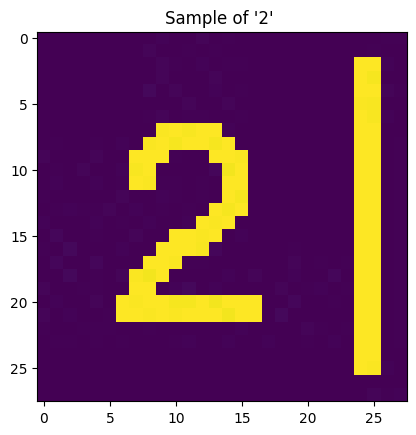
\includegraphics[width=2in]{2.png}
        \captionof{figure}{A sample of image '2'}
        \label{fig:figure_label}
    \end{center}
    Due to such noise the accuracy of these models in recognizing the Sudoku Digits decreases which is the most essential part of the models performance. The models performance on the training data can be good, but after testing on real sudoku images the model's performace was subpar.
     

%\end{minipage}

%\begin{minipage}[t]{0.5\textwidth}


So 'Printed Digit Dataset' was used.It Contains around 3000 images of digitally printed numeric dataset.
    Each image is of dimension 28x28 and is grayscale.
This dataset was purposely created for sudoku digits classification hence it shows blank image for 0 (zeros).
  \section{Procedure}
  \subsection{Image Processing}
  \subsubsection{Detecting Contours}
  
  Contours are used for extracting the Sudoku image from the raw image.First the image is converted to grayscale.
  Then for detecting contours, first gaussian blur\cite{opencv_smoothing} was used on the image along with thresholding\cite{opencv_thresholding} with the output being as shown in Figure 2. This the essential step for detecting contours.\cite{opencv_contours}
  Once the contuours are detected, the sudoku image can be extracted by using the biggest external contour.
   \begin{center}
        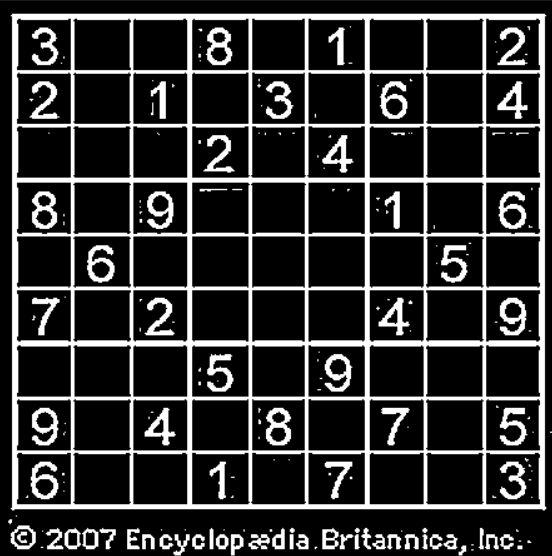
\includegraphics[width=2in]{thresholding.png}
        \captionof{figure}{Thresholding on a sample sudoku image}
        \label{fig:figure_label}
    \end{center}
    \subsubsection{Extracting Individual Cells}
    There are a total of 81 cells to be extracted, which will then be sent to the model to detect digits. As the image is an NxN dimensional array, it was split into 9 rows and columns using horizontal split and vertical split\cite{split_array} thereby creating 81 different boxes.
    
\newpage
\twocolumn
\subsection{Training the Model}
The Final Model had the following layers : 
\begin{itemize}
    \item 2x Convolutional Layers
    \item 2x MaxPooling Layers
    \item 2x Dense Layers (relu)
    \item 1x Dense Output Layer (softmax)
\end{itemize}
A dropout layer was added after the final maxpooling layer, to prevent overfitting. Early Callback was also implemented to prevent overfitting the data, as the data size was low. Before the dense layer, the Flatten layer was implemented to flatten the array to a single dimension for input in Dense Layers\cite{mnist}. 'Adam' optimizer was used along with 'Categorical Cross Entropy' as a loss function.
The model gave an accuracy of 98.25\% on the validation dataset(Figure 3).The model was then Serialized and saved for future use.
\begin{center}
        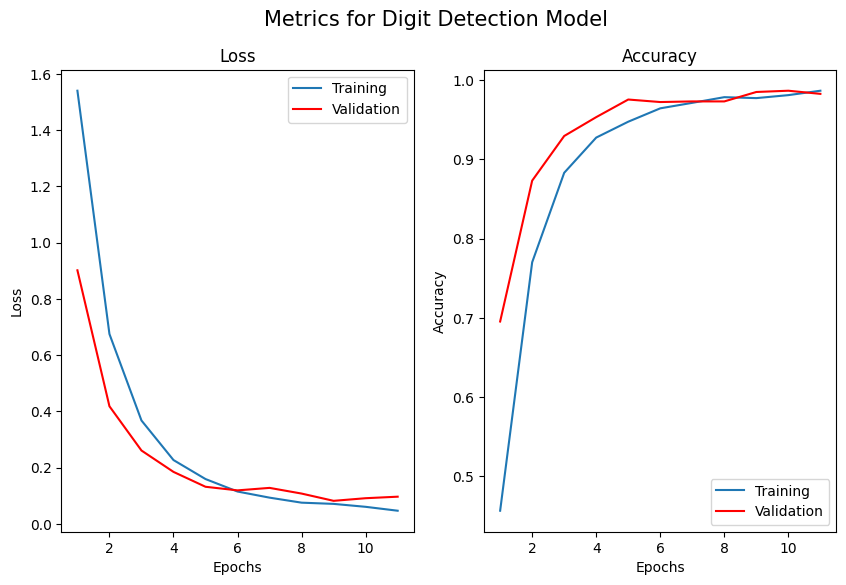
\includegraphics[width=3in]{model.png}
        \captionof{figure}{Metrics of the model}
        \label{fig:figure_label}
\end{center}
\subsection{Preprocessing Individual Cells and Detecting Digits}
As the extracted cells and the images the model was trained on were different, the cells needed to be preprocessed first before sending for detection. The images were reshaped into (1,28,28,1) dimensions each. Later 'Binary threshold'\cite{opencv_thresholding} was added along with 'bitwise not'\cite{arithmetic_op} to get the image into the same format as figure 1. Figure 4 and 5 show the initial and final images respectively.
\begin{center}
        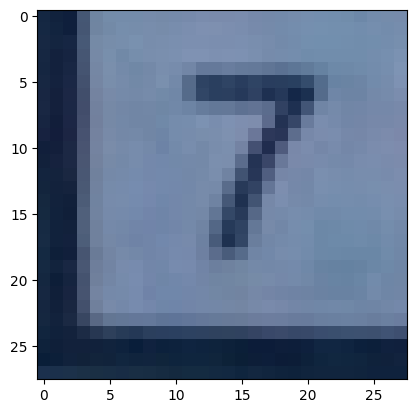
\includegraphics[width=2in]{c1.png}
        \captionof{figure}{Before Processing}
        \label{fig:figure_label}
\end{center}
\begin{center}
        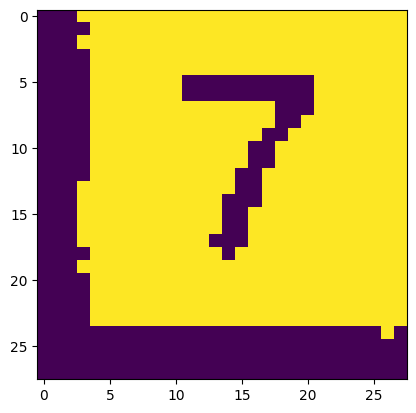
\includegraphics[width=2in]{c2.png}
        \captionof{figure}{After Processing}
        \label{fig:figure_label}
\end{center}
The Images were then scaled and individually sent to the model for Digit Detection. The digits were predicted from the results using argmax function from numpy\cite{tds_from_scratch}.The final result can be seen in figure 6.
\begin{center}
        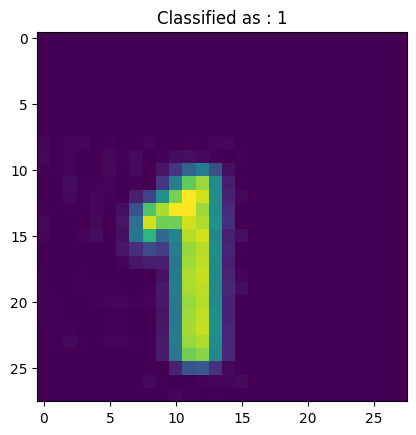
\includegraphics[width=2in]{classified.png}
        \captionof{figure}{Detected Image}
        \label{fig:figure_label}
\end{center}
\subsection{Solving the puzzle}
As the digits were detected, a 9x9 board(array) was created with those digits. There are now two methods to approach the problem : 
\begin{itemize}
    \item Simple Brute Force
    \item Backtracking Algorithm
\end{itemize}
Simple Brute Forcing may work to solve the board but has a disadvantage of requiring more computational time. Hence, a variation of Brute Force was used in solving called Backtracking Algorithm\cite{solver_algos}. Backtracking is a depth-first search (in contrast to a breadth-first search), because it will completely explore one branch to a possible solution before moving to another branch.
The Advantages of Backtracking are:
\begin{itemize}
    \item Simple to implement
    \item Guaranteed Solution (provided a valid Sudoku)\cite{solver_algos}
    \item Solving Time mostly unrelated to Degree of Difficulty
\end{itemize}
A separate python solver file was created for solving the board by implementing Backtracking Algorithm\cite{bt_twt}.The solved board was then sent back to main file for final processing.  
\subsubsection{Overlaying the results on Source Image}
A single image is created just containing the solved digits with identical height, width and perspective as the original image. The new image is then overlaid on top of the original image. The initial and final result is as shown in Figures 7 and 8 respectively.
\begin{center}
        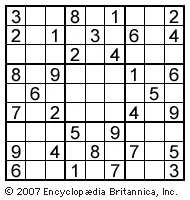
\includegraphics[width=2in]{2(1).png}
        \captionof{figure}{Original Image}
        \label{fig:figure_label}
\end{center}
\begin{center}
        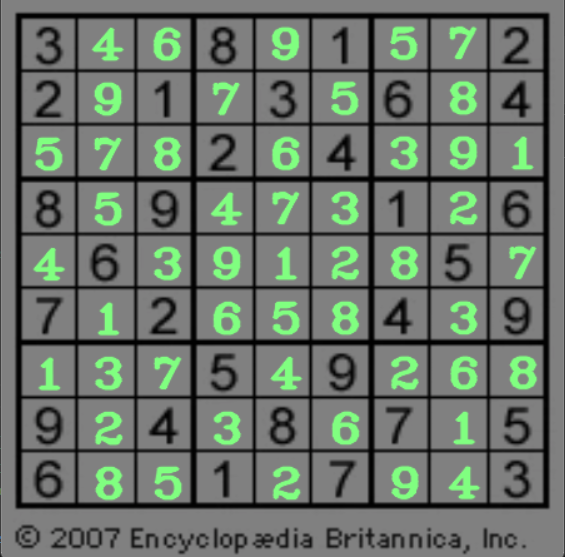
\includegraphics[width=2in]{img_after.png}
        \captionof{figure}{Solved Image}
        \label{fig:figure_label}
\end{center}
\section{Conclusion}
In conclusion, the application of image processing and machine learning in solving Sudoku puzzles has demonstrated a promising avenue for automating the traditionally manual tasks. By leveraging the capabilities of image processing to extract and recognize the Sudoku grid from an image and utilizing machine learning algorithms to analyze and solve the puzzle, the accuracy and efficiency of the system can be significantly improved.Moreover, the methods and techniques presented in the report can be of practical use to puzzle enthusiasts and developers of puzzle-solving software.
\section{Future Work and Improvements}
\begin{itemize}
    \item The accuracy of the model can be further improved by more augmentation of the pre-existing data or by using a different more dynamic dataset
    \item The model can be deployed on a web-based application by using Flask\cite{flask} or on an Android Device using Buildozer\cite{buildozer}
    \item The Sudoku puzzle once detected can be solved using more efficient Algorithms\cite{solver_algos}
    
\end{itemize}

%\end{minipage}
%\end{multicols}


%%{\color{gray}\hrule}
\begin{minipage}[t]{0.6\textwidth}
\section{Background and Pre-requisites}
The code is divided into different sections for easier understanding, with that said, having intermediate knowledge of python would be beneficial for understanding and analysing the code.
Beyond Basic  ML, one should be well-versed  in  different types of layers used in a Neural Network.
Two main python libraries were used in this project : open-cv and tensorflow, familiarity with both would be highly beneficial.

\end{minipage}
%\begin{multicols}{2}
%\subsection{Subsection}
%\lipsum[1-3]
%\subsection{Subsection}
%\lipsum[1-2]
%\end{multicols}
%%{\color{gray}\hrule}
%\usepackage{graphicx}
\begin{minipage}[t]{0.6\textwidth}
    \section{Datasets}
    Various Datasets were tested with, namely : 
    \begin{itemize}
        \item MNIST Handwritten Digits Dataset
        \item EMNIST
        \item USPS
        \item SVHN
    \end{itemize}
    But all these datasets had a problem that the models trained on them don't translate well into detecting digits on a Sudoku grid as there's a lot of noise in each of the extracted cells or boxes as seen in Figure.1.
    \begin{center}
        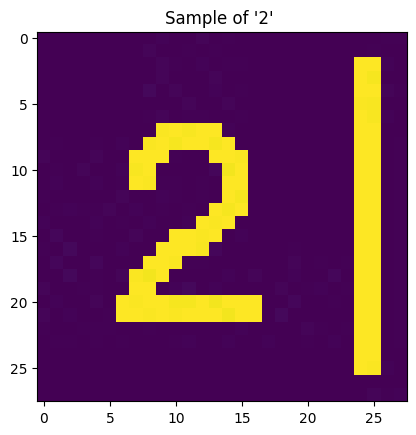
\includegraphics[width=2in]{2.png}
        \captionof{figure}{A sample of image '2'}
        \label{fig:figure_label}
    \end{center}
    Due to such noise the accuracy of these models in recognizing the Sudoku Digits decreases which is the most essential part of the models performance. The models performance on the training data can be good, but after testing on real sudoku images the model's performace was subpar.
    So 'Printed Digit Dataset' was used.It Contains around 3000 images of digitally printed numeric dataset.
    Each image is of dimension 28x28 and is grayscale. This dataset was purposely created for sudoku digits classification hence it shows blank image for 0 (zeros).

\end{minipage}





%{\color{gray}\hrule}
\begin{center}
\section{Section}
\textbf{Small description}
\end{center}
{\color{gray}\hrule}
\begin{multicols}{2}
\subsection{Subsection}
\lipsum[1]
\subsection{Subsection}
\lipsum[1-3]
\end{multicols}
%{\color{gray}\hrule}
\begin{center}
\section{Conclusions}
\end{center}
{\color{gray}\hrule}
\vspace{0.5cm}
\lipsum[1-2]
\onecolumn
\bibliographystyle{plain}
\bibliography{references}
%\bibliographystyle{plain}
%\bibliography{references}
\end{document}